PWM (Pulse Width Modulation) é um modulação baseada na conversão linear de um valor em escala de tensão para outro em escala de \emph{Duty Cicle} aplicado a uma onda quadrada de amplitude qualquer. Este tipo de modulação é essencial em controladores de circuitos de potência, já que através desta modulação é possível controlar um dispositivo de chaveamento como um Mosfet,  de modo que a tensão média sobre uma dada carga esteja diretamente relacionada com \emph{Duty Cicle} do chaveamento.  

\section{Modos de Funcionamento}

Para criar uma modulação PWM é necessário criar uma onda portadora cuja a amplitude do sinal varie no tempo permitindo comparar a sua amplitude com o do sinal modulante. O sinal modulante nada mais é do que o sinal ao qual se deseja converter em escala de \emph{Duty Cicle}. Normalmente a onda portadora utilizada neste tipo de modulação é a onda triangular ou a onda dente de serra.
  
A modulação PWM é realizada através da comparação direta entre o modulo do sinal modulante e a onda portadora em cada instante de tempo. A implementação desta modulação analogicamente é bem simples, basta conectar o sinal modulante na porta positiva e o sinal da portadora na porta negativa de amplificador operacional na configuração comparador, a saída do amplificador será o sinal modulado.

Já para a implementação digital deste método pode ser feito através uma comparação direta entre os módulos dos dois sinais. Quando o modulo do sinal modulante for maior do que o  módulo da portadora  o sinal modulado vai para nível alto. Porém quando o módulo do sinal modulante for menor do que o módulo da portadora o sinal  modulado vai para zero. A grande diferença da implementação digital é que o sinal da portadora é gerado internamente através de um contador, que pode trabalhar no modo de contagem \emph{Down}, \emph{Up} ou \emph{UpDown}.

Quando o sinal da portadora é gerado através de um contador \emph{Down} ou \emph{Up}  a frequência do sinal modulado será igual a frequência de contador dividido pelo numero máximo de contagens. Já quando o sinal da portadora é gerador por um contador\emph{UpDown} a frequência do sinal modulado será igual a frequência do contador dividido por duas vezes o numero máximo de contagens. Sendo que o numero máximo de contagens deve ser maior ou igual ao modulo do sinal modulante. A Figura \ref{fig:Down} e a Figura \ref{fig:UpDown} apresentam melhor o modo como a geração de PWM é realizada digitalmente.  

\begin{figure}[H]
	\centering
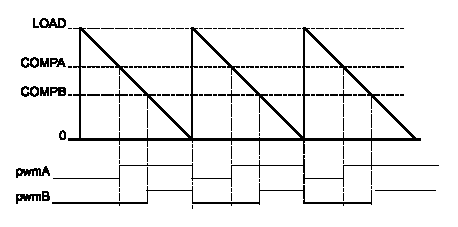
\includegraphics[width=0.8\textwidth] {figuras/Down.eps}
	\caption{PWM modo Down \cite{DATASHEET_TIVA}}
	\label{fig:Down}
\end{figure}

\begin{figure}[H]
	\centering
	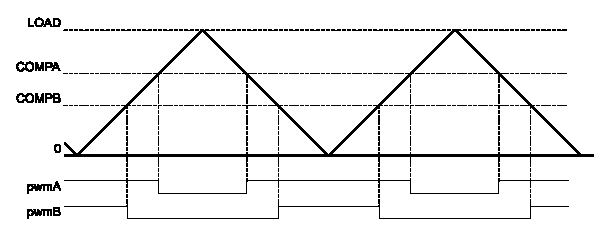
\includegraphics[width=0.8\textwidth] {figuras/UpDown.eps}
	\caption{PWM modo Down \cite{DATASHEET_TIVA}}
	\label{fig:UpDown}
\end{figure}

Tanto na Figura \ref{fig:Down} quanto na Figura \ref{fig:UpDown} os valores de \emph{LOAD}, \emph{COMPA}, \emph{COMPB}, \emph{pwmA} e \emph{pwmB} são referentes aos registradores presente do Tiva - TM4C1294NCPD, responsáveis pela modulação PWM. Tais registradores serão melhor abordados na próxima seção.  

\section{PWM do TM4C1294NCPDT}

\begin{figure}[H]
	\centering
	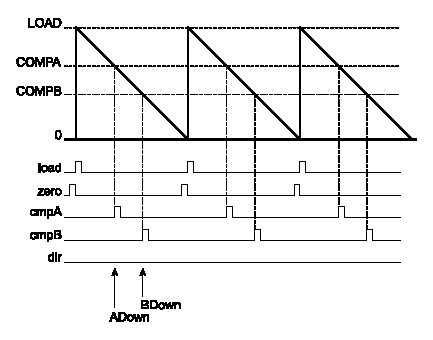
\includegraphics[width=0.8\textwidth] {figuras/PWMCountDownMode.eps}
	\caption{PWM modo Down \cite{DATASHEET_TIVA}}
	\label{fig:PWMCountDownMode}
\end{figure}

\begin{figure}[H]
	\centering
	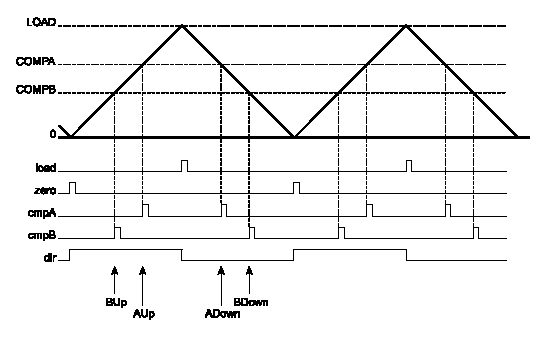
\includegraphics[width=0.8\textwidth] {figuras/PWMCountUpDownMode.eps}
	\caption{PWM modo Down \cite{DATASHEET_TIVA}}
	\label{fig:PWMCountUpDownMode}
\end{figure}